\chapter{Sets}
\label{ch:new_sets}

Here are the \href{file:///Users/umut/Desktop/slides.pdf}{lecture slides}.
%
Here is a the \href{file://paper.xml}{xml file}.
%
Here is a \video{https://www.youtube.com/watch?v=8QyE9D_3ezQ&list=WL&index=2&t=0s}{tango video.}


\begin{table}
\begin{tabular}{ll}
Here & there
\\
There * here
\end{tabular}
\caption{Potent stuff.}
\label{tab:potent}
\end{table}

\begin{figure}[h!]
\begin{center}
  \includegraphics[width=0.9\textwidth]{img/memory.png}
\end{center}
\caption{A More Concrete Memory Model}
\label{fig:C0-memory}
\end{figure}

\begin{question}
Here as a ref to a book \ref{TB/}.

Here is a nicer ref to  abook \href{TB/}{ref to a book}.
This is Part~3 of Sipser's textbook %\href{https://www.google.com/search?q=Sipser\%20Introduction\%20to\%20the\%20Theory\%20of\%20Computation}
%{Introduction to the Theory of Computation}.

\href{https://www.google.com/search?q=Sipser}{Introduction to the Theory of Computation}.

Here you can
\begin{itemize}
\item \download{/Users/umut/Desktop/paper.xml}{download an xml file}
\item \attach{/Users/umut/Desktop/paper.xml}{find attached the xml file.}
\item \href{file:///Users/umut/Desktop/paper.xml}{download an xml file via href}
\end{itemize}

Here are some cross-book references: 
\begin{itemize}
\item  Ref \ref{TB/sec:bg::graphs::basics}
\item Ref \ref{TB/ex:bg::graphs::basics::examples}
\item Ref \ref{TB/def:bg::graphs::basics::enumerable}
\item Ref \ref{TB/sec:bg::graphs::weighted}
\end{itemize}

Here are some local references: 
\begin{itemize}
\item Ref \ref{xy}
\item Ref \ref{ans:new_sets:::downloads}
\item Ref \ref{sec:new_sets::math}
\item Ref \ref{adt:sets} 
\item Ref \ref{syn:sets}
\end{itemize}

\end{question}

\begin{answer}
\label{ans:new_sets:::downloads}
Here you can \download{/Users/umut/Desktop/paper.xml}{download an xml file}
Here you can \attach{/Users/umut/Desktop/paper.xml}{find attached the xml file}
And post downlead.
\end{answer}

\begin{preamble}[][cover = image; sound = sound.mpg; this = that.jpg]
  Sets are both a mathematical structure and an abstract datatype
  supported by many programming languages.  This chapter presents an ADT for
  finite sets of elements taken from a fixed domain and several cost models, including one based on \href{TB/ch:bst::adt}{balanced binary search trees}.

 
\begin{itemize}
\item
\lstinline'xyz'
\item
\lstinline`xyz`
\item
\lstinline!abc! 
\end{itemize}
\end{preamble}

\begin{gram}[Table title][cover = coverimage.pdf; sound=playthis.mp3]
\begin{tabular}{lll}
Here & there & where? 
\\ \hline
where & there & here? 
\\ \hline
\end{tabular}
\end{gram}


\begin{table}
\[
\begin{array}{lll}
\mbox{Here} & \mbox{there} & \mbox{where?} 
\\ \hline
\mbox{where} & \mbox{there} & \mbox{here?} 
\\ \hline
\end{array}
\]
\end{table}

\begin{figure}
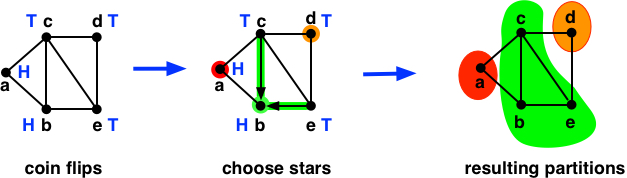
\includegraphics{star-find0.jpg}
\caption{Some image above.}
\end{figure}


\begin{table}
\includegraphics{Something}
\caption{Some image above.}
\end{table}

  \section{Motivation}
\label{sec:new_sets::math}


\begin{gram}
\begin{quote}
``A \emph{set} is a gathering together into a whole of definite, distinct
objects of our perception or of our thought---which are called \emph{elements}
of the set.''\\[.1in] Georg Cantor, from ``Contributions to the founding of the theory of transfinite numbers.''
\end{quote}

Set theory, founded by Georg Cantor in the second half of the
nineteenth century, is one of the most important advances in
mathematics.  From it came the notions of countably vs. uncountably
infinite sets, and ultimately the theory of computational
undecidability, i.e. that computational mechanisms such as the
$\lambda$-calculus or Turing Machine cannot compute all functions.
Set theory has also formed the foundations on which other branches of
mathematics can be formalized.  Early set theory, sometimes referred
to as na\"{\i}ve set theory, allowed anything to be in a set.  This
led to several paradoxes such Russell's famous paradox:
  \[\mbox{let } R = \csetf{x}{x \not\in x}, \mbox{ then } R \in R \iff R \not\in R
\;.\] Such paradoxes were resolved by the development of axiomatic set
theory.  Typically in such a theory, the universe of possible elements
of a set needs to be built up from primitive notions, such as the
integers or reals, by using various composition rules, such as
Cartesian products.
\end{gram}
\begin{gram}
x
\end{gram}

%% \begin{gram}[10][Choices]
%% Select any one of the following.
%% \begin{anychoice}
%% \choice a
%% \choice $b = y^2$
%% \choice* c
%% \choice* d
%% \choice e
%% \end{anychoice}
%% \end{gram}

\begin{gram}
\label{xy}
Our goals in this book are much more modest than trying to understand set theory and its many interesting implications.  Here we simply recognize that in algorithm design sets are a very useful data type in their own right, but also in building up more complicated data types, such as graphs.  Furthermore particular classes of sets, such as mappings (or tables), are themselves very useful, and hence deserve their own interface. 
%
We discuss tables \href{TB/ch:tables}{in the next chapter.}

\end{gram}

\begin{gram}
Other chapters cover data structures on binary search trees
(\chref{bst::adt}) and hashing (\chref{hash-tables}) that can be used for
implementing the sets and tables interfaces. 
%
Applications of sets and tables include \href{TB/ch:graphs::graphs}{graphs}.
%
We note that \href{TB/ch:sequences::adt}{sequences} are a particular type of table---one where the domain of the tables are the integers from $0$ to $n-1$.  
\end{gram}

% \begin{gram}
% %\begin{comment}
% Returning to the discussion in the first paragraph about paradoxes in 
% set theory: in our presentation we define sets as elements from 
% particular universes, so as long as these universes are built up in a 
% certain way, we avoid such paradoxes.  However, we put an additional
% restriction on sets (and tables).  In particular, although we allow
% for infinite universes (countable or uncountable) we limit ourselves
% to finite sized sets.  This means we certainly do not capture all set
% theory, but the assumption makes everything computationally feasible.
% Representation of infinite sets is an interesting research topic but
% beyond the scope of this book.
% \end{gram}




       \section{Sets ADT}

\begin{datatype}[Sets]
\label{adt:new_sets} 

For a universe of elements $\uuu$ that support equality (e.g. the integers or strings), the 
\adt{SET} abstract data type is a type $\sss$ representing the power 
set of $\uuu$ (i.e., all subsets of $\uuu$) limited to sets of finite 
size, along with the functions below. 
{\normalsize
\input{./sets-and-tables/sig-sets}
}
Where $\tynat$ is 
the natural numbers (non-negative integers) and $\bbb = \{\texttt{true},
\texttt{false}\}$.
%; for a set $A$ of type $\sss$.
%, $\means{A}$ denotes the  (mathematical) set of keys in the set.
\end{datatype}

\begin{syntax}[Sets] 
\label{syn:new_sets}
In \pml{}  we use the standard set notation $\cset{e_o,e_1,\cdots,e_n}$ to
  indicate a set.  The notation $\emptyset$ or $\cset{}$ refers to an
  empty set. We also use the conventional mathematical syntax for set
  functions such as $|S|$ (size), $\cup$ (union), $\cap$
  (intersection), and $\setminus$ (difference).  In addition, we use
  set comprehensions for $\cdvar{filter}$ and for constructing sets from
  other sets.
\end{syntax}

\begin{gram}
  The objects that are contained in a set are called~\defn{members}~or the~\defn{elements}~of the set.  Recall that a~\defn{set}~is a collection of distinct objects.  This requires that
  the universe $\uuu$ they come from support equality.  It might seem that
  all universes support equality, but consider functions.  When are
  two functions equal?   It is not even decidable whether two
  functions are equal.   From a practical matter, there is no way to
  implement sets without an equality function over potential
  elements.   In fact efficient implementations additionally require
  either a hash function over the elements of $\uuu$ and/or a total ordering.
\end{gram}

\begin{gram}
The Set ADT consists of basic functions on sets.  
%
The function $\cdvar{size}$ takes a set and returns the number of elements
in the set.
% 
The function $\cdvar{toSeq}$ converts a set to a sequence by ordering the
elements of the set in an unspecified way. 
%
Since elements of a set do not necessarily have a total ordering, the
resulting order is arbitrary.
%
This means that $\cdvar{toSeq}$ is possibly non-deterministic---it could
return different orderings in different implementations.
%, or even on different runs of the same implementation.
%
We specify $\cdvar{toSeq}$ as follows
\[
\cdvar{toSeq}~(\{x_0,x_1,\ldots,x_n\} : \sss): seq = \cseq{x_0,x_1,\ldots,x_n}
\]
where the $x_i$ are an arbitrary ordering. 
\end{gram}


\begin{gram}
Several functions enable constructing sets.
%
The function $\cdvar{empty}$ returns an empty set:
%
\[
\cdvar{empty} : \sss = \emptyset
\]
%
The function $\cdvar{singleton}$ constructs a singleton set from a given
element.
%
\[
\cdvar{singleton} (x : \uuu) : \sss = \{x \}
\]
%
The function $\cdvar{fromSeq}$ takes a sequence and returns a set consisting of the
distinct elements of the sequence, eliminating duplicate elements.
%
We can specify $\cdvar{fromSeq}$ as returning the range of the sequence
$A$ (recall that a sequence is a partial function mapping from natural numbers
to elements of the sequence).
%
\[
\cdvar{fromSeq}~(a : seq) : \sss = \cdvar{range}~a
\]
%
\end{gram}

\begin{gram}
%
Several functions operate on sets to produce new sets.
%
The function $\cdvar{filter}$ selects the elements of a sequence that
satisfy a given Boolean function, i.e., 
%
\[
\cdvar{filter}~(f : \uuu \ra \tybool)~(a : \sss) : \sss = \{ x \in a \sucht f(x)\} .
\]
%
The functions $\cdvar{intersection}$, $\cdvar{difference}$, and $\cdvar{union}$
perform the corresponding set operation on their arguments:
%
\[
\begin{array}{l}
\cdvar{intersection}~(a : \sss)~(b : \sss) : \sss = a \cap b\\
\cdvar{difference}~(a  : \sss)~(b : \sss) : \sss = a \setminus b\\
\cdvar{union}~(a : \sss)~(b : \sss) : \sss = a \cup b
\end{array}
\]
%
We refer to the functions  $\cdvar{intersection}$, $\cdvar{difference}$, and $\cdvar{union}$
as \defn{bulk updates}, because they allow updating with a large set
of elements ``in bulk.''
\end{gram}

\begin{gram}
The functions $\cdvar{find}$, $\cdvar{insert}$, and $\cdvar{delete}$ are singular
versions of the bulk functions $\cdvar{intersection}$, $\cdvar{union}$, and
$\cdvar{difference}$ respectively.
%
The $\cdvar{find}$ function checks whether an element is in a set---it is
the basic membership test for sets.
%
\[
find~(a  : \sss)~(x : \uuu) : \tybool = \left\{
                \begin{array}{ll}
                \cd{true} & \cd{if}~x \in A \\
                \cd{false} & \cd{otherwise}
                \end{array} \right.
\]
%
We can also specify the $\cdvar{find}$ function is in terms of set
intersection:
\[
find~(a : \sss)~(x : \uuu) : \tybool = \csetsize{a \cap \cset{x}} = 1.
\]
%
The functions $\cdvar{delete}$ and $\cdvar{insert}$ 
%
delete an existing element from a set, and
%
insert a new element into a set,
%
respectively:
%
\[
\begin{array}{l}
\cdvar{delete}~(a  : \sss)~(x  : \uuu) : \sss = a \setminus \cset{x}.\\
\cdvar{insert}~(a : \sss)~(x : \uuu) : \sss = a \cup \cset{x}
\end{array}
\]
%
\end{gram}

\begin{gram}
Iteration and reduction over sets can be easily defined by converting
them to sequences, as in

\[
\begin{array}{l}
\cdvar{iterate}~f~x~a = \cdvar{Sequence.iterate}~f~(\cdvar{toSeq}~a)\\
\cdvar{reduce}~f~x~a = \cdvar{Sequence.reduce}~f~(\cdvar{toSeq}~a)
\end{array}
\]
\end{gram}

% The next two functions enable aggregating over sets, via iteration 
% and reduction.
% %
% The function $\cdvar{iterate}$ can be used to iterate over a set while
% accumulating information.
% %
% The function takes an initial value $x$, a function~$f$, and a
% set~$A$, and iterates over the elements of $A$ in some unspecified,
% possibly non-deterministic, order, to produce a final value.
% %
% \[
% \begin{array}{l}

% \begin{array}{ll}
% x & \mbox{if}~ \csetsize{A}= 0\\
% \cdvar{iterate}~f~(f(v, y))~(A \setminus \cset{y}) & \mbox{otherwise, where}~y \in A.
% \end{array}
% \right.
% \end{array}
% \]
% %
% The function $\cdvar{iterate}$ computes its final result by computing a
% new state for each element of the set $A = \cset{a_0, \ldots a_n}$
% \[
% \begin{array}{lcl}
% x_0 & = & x
% \\
% x_1 & = & f(x_0,a_0)
% \\
% x_2 & = & f(x_1, a_1)
% \\
% & \vdots &
% \\
% x_{n} & = & f(x_{n-1},a_n).
% \end{array}
% \]


% To perform a reduction over a set, the ADT supplies the  $\cdvar{reduce}$ function.
% %
% The function takes an associative binary function~$f$ along with the
% left identity element for the function~$id$, and applies~$f$ to the
% elements in the set to produce the ``sum'' of the elements.
% %
% The identity of~$f$ satisfies the constraint that $f(id,x) = x$ for
% all $x \in \uuu$.
% %
% For a set $A = \cset{a_0, \ldots, a_n}$,
% we can define the behavior of $\cdvar{reduce}$ inductively as follows.
% %
% \[
% \begin{array}{l}
% \cdvar{reduce}~(f : \uuu * \uuu \ra \uuu)~(id: \uuu)~(A: \sss) : \uuu
% \\
% ~~~~~=
% \left\{
% \begin{array}{ll}
% id & \mbox{if}~\csetsize{A}= 0\\
% A[0] & \mbox{if}~\csetsize{A}= 1\\
% f(x,y) & \mbox{if}~\csetsize{A}= 2,~\mbox{and}~A = \cset{x,y}\\
% f(\cdvar{reduce}~f~id~\cset{a_0, \ldots, a_{m}}
% \\
% ~~~\cdvar{reduce}~f~id~\cset{a_{m+1}, \ldots, a_n} & \mbox{otherwise, where}~m = \lceil n/2 \rceil.
% \end{array}
% \right.
% \end{array}
% \]
% \end{gram}

% %
% \begin{todo}

% The relation between reduce and iterate can be discussed.  it
%   requires commutativity. THe following copied from seq's

% The function \cdvar{reduce} is more restrictive than \cdvar{iterate} since
% it is the same function but with extra restrictions on its input
% (i.e. that~$f$ be associative, and $id$ is a left identity).
% %
% If the function $f$ is associative, then we have
% \[
% \cdvar{reduce}~f~id~A = \cdvar{iterate}~f~id~A.
% \]
% %
% \end{todo}
\begin{gram}
Notice that in the Set ADT although the universe $\uuu$ is potentially
infinite (e.g. the integers), $\sss$ only consists of finite sized
subsets.
%
Unfortunately this restriction
means that the interface is not as powerful as general set theory, but
it makes computation on sets feasible.  A consequence of this
requirement is that the interface does not include a function that
takes the complement of a set---such a function would generate an
infinite sized set from a finite sized set (assuming the size of $U$
is infinite).
\end{gram}

\begin{exercise}
Convince yourself that there is no way to create an infinite sized set
using the interface and with finite work.
\end{exercise}

\begin{example}
  Some functions on sets:
  \[
\begin{array}{lcl}
|\cset{a,b,c}| & = & 3\\
\csetf{x \in \cset{4,11,2,6}}{x < 7} & = &
\cset{4,2,6}\\
\cdvar{find}~\cset{6,2,9,11,8} 4  & = & \cfalse\\
\cset{2,7,8,11} \cup \cset{7,9,11,14,17} & = &
\cset{2,7,8,9,11,14,17}\\
\cdvar{toSeq}~\cset{2,7,8,11} & = & \cseq{8,11,2,7}\\
\cdvar{fromSeq}~\cseq{2,7,2,8,11,2} & = & \cset{8,2,11,7}
\end{array}
\]
\end{example}

\begin{remark}
You may notice that the interface does not
contain a $\cdvar{map}$ function.  If we interpret $\cdvar{map}$, as in sequences, to take in a collection, apply some
function to each element and return a collection of the same size,
then it does not make sense for sets.
Consider a function that always returns $0$.  Mapping this over a set would
return all zeros, which would then be collapsed into a singleton set, containing
exactly $0$.  Therefore, such a $\cdvar{map}$ would allow reducing the set of
arbitrary size to a singleton.
\end{remark}

\begin{remark}
Most programming languages either support sets directly (e.g., Python and Ruby)
or have libraries that support them (e.g., in the C++ STL library and Java
collections framework).  They sometimes have more than one implementation of
sets.  For example, Java has sets based on hash tables and balanced trees.
Unsurprisingly, the set interface in different libraries and languages differ in
subtle ways.  So, when using one of these interfaces you should always read the
documentation carefully.
\end{remark}


\section{Cost of Sets}

\begin{gram}
Sets can be implemented in several ways. 
%
If the elements of a set are drawn from natural numbers, it is sometimes possible and effective to represent the set as an array-based sequence.
%
If the elements accept a hash function, then hash-tables can be used to store the elements in a sequence.  This approach is commonly used in practice and is quite efficient in terms of work and space.
%
Finally, if the elements don't accept a hash function but accept a comparison operator that can totally order all elements, then sets can be represented by using binary search trees.
%
All of these approaches assume an equality function on the elements (with natural numbers, the equality coincides with the equality on natural numbers).

%% An interesting aspect of both of these implementations is that they
%% require more than just equality on the element (or the universe $\uuu$):
%% an implementation based on balanced search trees requires a total
%% ordering on the elements of $\uuu$ and hence a comparison; and an
%% implementation based on hashing does not require comparison, but
%% requires the ability to hash the elements of $\uuu$.  
%
% For the purposed of the ADT, we consider the functions for equality,
% comparison, and hashing, to be implicitly defined on the universe
% $\uuu$.
\end{gram}

\begin{flex}
\label{sets:cluster:arraysets}

\begin{costspec}[Array Sets for Enumerable Sets]
\label{cost:new_sets::arrayseqs}

Let the universe $U$ be defined as the set 
%
$\{ 0, 1, \ldots, u-1 \}$
%
for some $u \in \nats$.
%
We can represent \defn{enumerable sets} of the form $S \subseteq U$ by using a sequence that indicates for each $i \in U$ whether $i \in S$ or not.
%
Using array sequences, operations on enumerable sets can be implemented according to the following cost specification.
 
\input{./sets-and-tables/cost-sets-arrayseqs}
\end{costspec}


\begin{example}
Consider a graph whose vertices are labeled by natural numbers up to $8$.  We can a graph whose vertices are
%
$\{ 0, 2, 4, 6 \}$ 
%
with the sequence:
%
$\cseq{ 1, 0, 1, 0, 1, 0, 1, 0 }.$ 
\end{example}

\end{flex}


\begin{gram}[Tree Representation for Sets]
If the elements in the universe $\uuu$ accept a comparison function 
that defines a total order over $\uuu$, then we can use a balanced binary search tree to represent sets.
%
This representation allows us to implement the Sets ADT reasonably efficiently.
%
For the specification \href{cost:new_sets::trees}{specified below}, we assume that the comparison function requires constant work and span.  
%
\end{gram}

\begin{costspec}[Tree Sets]
\label{cost:new_sets::trees}
\input{./sets-and-tables/cost-sets-tree}
\end{costspec}

\begin{gram}
Let's consider these cost specifications in some more detail.  The
cost for $\cdvar{filter}$ is effectively the same as for sequences, and
therefore should not be surprising.  It assumes the function $f$ is
applied to the elements of the set in parallel.  The cost for the
functions $\cdvar{find}$, $\cdvar{insert}$, and $\cdvar{delete}$ are
what one might expect from a balanced binary tree implementation.
Basically the tree will have $O(\lg n)$ depth and each function will
require searching the tree from the root to some node.  We cover
such an implementation in \chref{bst::parametric}.
\end{gram}

% \begin{notesonly}
% TODO:

% filter cost of logn is actually not so easy to achieve by
% using split and join.  it seems that we would need
% pipelining/futures. the natural implementation yields log2n.

% similarly with union et al, the straigtfoward implementation
% yields log2n.  We need pipelining/futures to achieve logn.
% \end{notesonly}

\begin{gram}
  The work bounds for the bulk functions ($\cdvar{intersection}$,
  $\cdvar{difference}$, and $\cdvar{union}$) may seem confusing,
  especially because of the expression inside the logarithm.  To shed
  some light on the cost, it is helpful to consider two cases, the
  first is when one of the sets is a single element and the other when
  both sets are equal length.  In the first case the bulk functions
  are doing the same thing as the single element functions
  $\cdvar{find}$, $\cdvar{insert}$, and $\cdvar{delete}$.  Indeed if
  we implement the single element functions on a set $A$ using the
  bulk ones, then we would like it to be
  the case that we get the same asymptotic performance.  This is
  indeed the case since we have that $m = 1$ and $n = |A|$, giving:

\[W(n) \in O\left(\lg \left(1 + \frac{n}{1}\right)\right) 
= O(\lg n)~.\]

Now let's consider the second case when both sets have equal length,
say $n$.   In this case we have $m = n$ giving
\[
W(n) \in O\left(n \cdot \lg \left(1+\frac{n}{n}\right)\right) = O(n).
\]
\end{gram}

% \begin{notesonly}
% \cdvar{find} $\leftrightarrow$ \cdvar{intersection}\\
% \cdvar{insert} $\leftrightarrow$ \cdvar{union}\\
% \cdvar{delete} $\leftrightarrow$ \cdvar{difference}

% \begin{lstlisting}[numbers=none]
% fun intersection$(S_1,S_2)$ = filter (fn $x$ => find $x$ $S_1$) $S_2$
% fun intersection$(S_1,S_2)$ = 
%   iter (fn $(S,x)$ => if find$(S_1,x)$ then insert$(S,x)$ else $S$)
%        $\emptyset$ $S_2$
% fun difference$(S_1,S_2$ = iter delete S_1 S_2
% fun union$(S_1,S_2)$ = iter insert S_1 S_2@\vspace{.1in}@
% \end{lstlisting}
% \end{notesonly}

\begin{gram}
We can implement $\cdvar{find}$, $\cdvar{delete}$, and $\cdvar{insert}$ in terms of
the functions $\cdvar{intersection}$, $\cdvar{difference}$, and $\cdvar{union}$
(respectively) by making a singleton set out of the element that we
are interested in.
%
Such an implementation would be asymptotically efficient, giving us
the work and span as the direct implementations.
%

Conversely, we can also implement the bulk functions in terms of the
singleton ones by iteration.
%
Because it uses iteration the resulting algorithms are
sequential and also work inefficient.
%
For example, if we implement $\cdvar{union}$ by inserting
$n$ elements into a second set of $n$ elements, the cost would be $O(n
\lg n)$.  
%
We would obtain a similar bound when implementing
$\cdvar{difference}$ with $\cdvar{delete}$, and $\cdvar{intersection}$ with
$\cdvar{find}$ and $\cdvar{insert}$.
%
For this reason, we prefer to use the bulk functions $\cdvar{intersection}$, $\cdvar{difference}$, and $\cdvar{union}$ instead
of $\cdvar{find}$, $\cdvar{delete}$, and $\cdvar{insert}$ when possible.
\end{gram}

% \begin{notesonly}
% \begin{question}
% Why can we not make the implementations of the bulk functions parallel
% by replacing \cdvar{iter} with \cdvar{reduce}.
% \end{question}
% Unfortunately we cannot implement a parallel version of the bulk
% functions by replacing \cdvar{iter} with \cdvar{reduce} since the
% combining functions being used are not associative.
% \end{notesonly}

\begin{example}
\label{ex:new_sets::fromseq-imp}
We can  convert a sequence to a set by inserting the elements
one by one as follows
\[
\cdvar{fromseq}~a = \cdvar{Seq.iterate}~\cdvar{Set.insert}~~\emptyset~a.
\]

This implementation is sequential and work inefficient. 
%
We can write a parallel and work-efficient function as follows
\[
\cdvar{fromSeq}~a = \cdvar{Seq.reduce}~\cdvar{Set.union}~~\emptyset~~\cseq{\cset{x} : x \in a}.
\]

\end{example}


